%\VignetteIndexEntry{Genometric Correlation}
%\VignetteIndexEntry{GenometriCorrelation}
%\VignetteIndexEntry{GenometriCorrelation}
%\VignettePackage{GenometriCorr}



\documentclass{article}

\usepackage{amsmath}

\usepackage[pdftex]{graphicx}
  % \graphicspath{{../pdf/}{../jpeg/}}
  % \DeclareGraphicsExtensions{.pdf,.jpeg,.png}
\usepackage{float}
\usepackage{inputenc}
\usepackage{natbib}
\usepackage{indentfirst}
\usepackage[font=small]{caption}
\usepackage{color}
\usepackage{Sweave}

%\usepackage{graphicx}

\begin{document}

\title{GenometriCorr (Genometric Correlation): an R package for spatial correlation of genome-wide interval datasets}
\author{Alexander Favorov\footnote{favorov@sensi.org}, Loris Mularoni, Leslie M. Cope, Andrey A. Mironov\\ Yulia Medvedeva, Vsevolod J. Makeev, Sarah J. Wheelan}

\maketitle

\section{Introduction}

\newcommand{\picscale}{0.5}

\subsection{Genometric layouts; independence or correlation}
\subsubsection{Using distance as a proxy for functional correlation}
High-throughput sequencing has become a popular and ever more affordable method in molecular biology and clinical experiments, and will soon become a routine laboratory technique. Sequencing reads are mapped to a reference genome and the results are often drawn as points along lines representing chromosomes, with the layout of the points reflecting the physical distance between mapped reads. While this depiction is a convention, it is based on a longstanding belief that proximity on a chromosome implies potential functional interaction.

If sequencing results are analyzed as points on a line, we can measure the physical distance between sequencing results and annotated genomic features. Deviations in these measurements from the expected distributions indicate associations (or anti-associations) that may be biologically interesting. While it is not difficult to judge these associations by eye, a genome-wide assessment of spatial correlations is impractical to do manually.

Many, though certainly not all, functional relationships in genetics are based on proximity. For example, a promoter will be near the 5' end of the gene that it controls, a splicing control signal will be near splice sites, transcription factor binding sites will cluster where the transcription factors bind to regulate gene activity, and more. Measuring the proximity of a set of points on the genome to various genomic features will direct future experiments.

Note that this type of correlation is not intended to give final results, but to generate testable hypotheses.


Genomic intervals are anything that can be stored as a chromosome number, start, and end. Strands are not considered but could be managed by subsetting the data. Genomic intervals can be represented as blocks on a line:
\begin{figure*}[h]
	\centering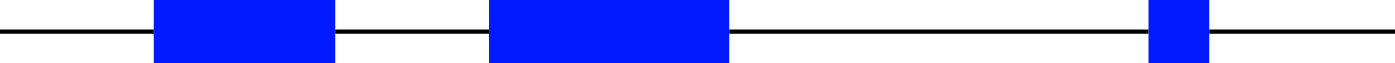
\includegraphics[scale=\picscale]{png/fig1}
	\caption{Genomic intervals}
\end{figure*}


\subsubsection{Intervals can be correlated or independent}

If we have two types of features, they can be correlated, or they can be independent. If the features are independent, the locations of one type of feature are randomly positioned with respect to the other, while if they are correlated, the locations of the feature types will, on average, follow a recognizable pattern; the features can be a relatively constant distance apart, they can be consistently near or far away from each other in genomic coordinates, or they can preferentially overlap (or only rarely overlap). Thus, if features are correlated, the locations of one type of feature give information about the positions of the other type of feature.
\begin{figure*}[h]
 \centering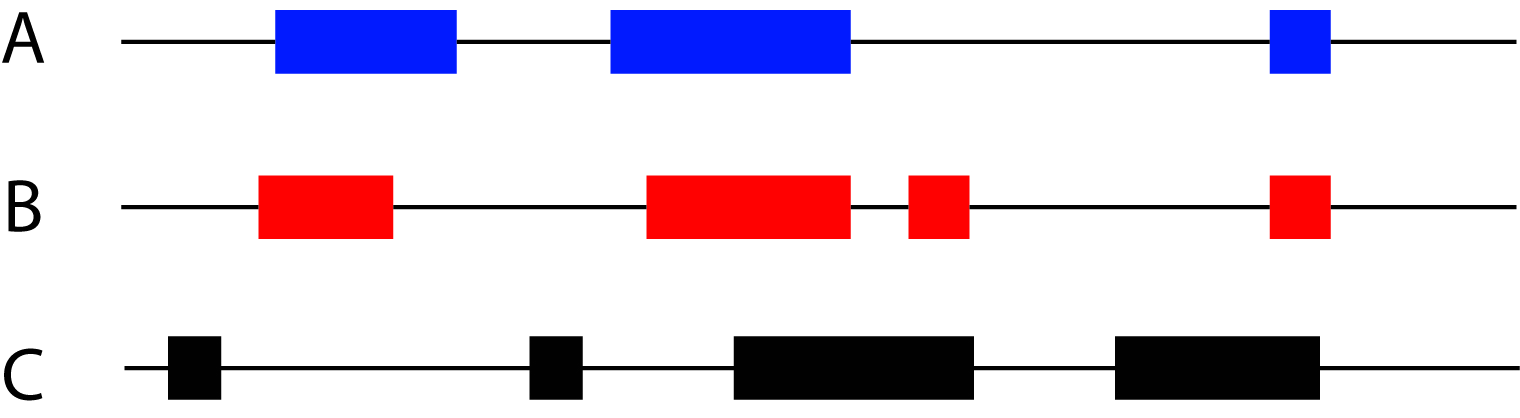
\includegraphics[scale=\picscale]{png/fig2}
 \caption{Three sets of genomic intervals. A and B are correlated, A and C are independent.}
\end{figure*}

\subsubsection{Correlation comes in many different flavors}
We will introduce some terminology for simplicity. The set of intervals whose positions are considered fixed in the genome is the reference set. The intervals whose positions are being tested to see whether they are related to the reference set in any way is the query set. Note that the comparison is thus asymmetric.

Figure 3 shows the basic question we are asking.

\begin{figure*}[h]
	\centering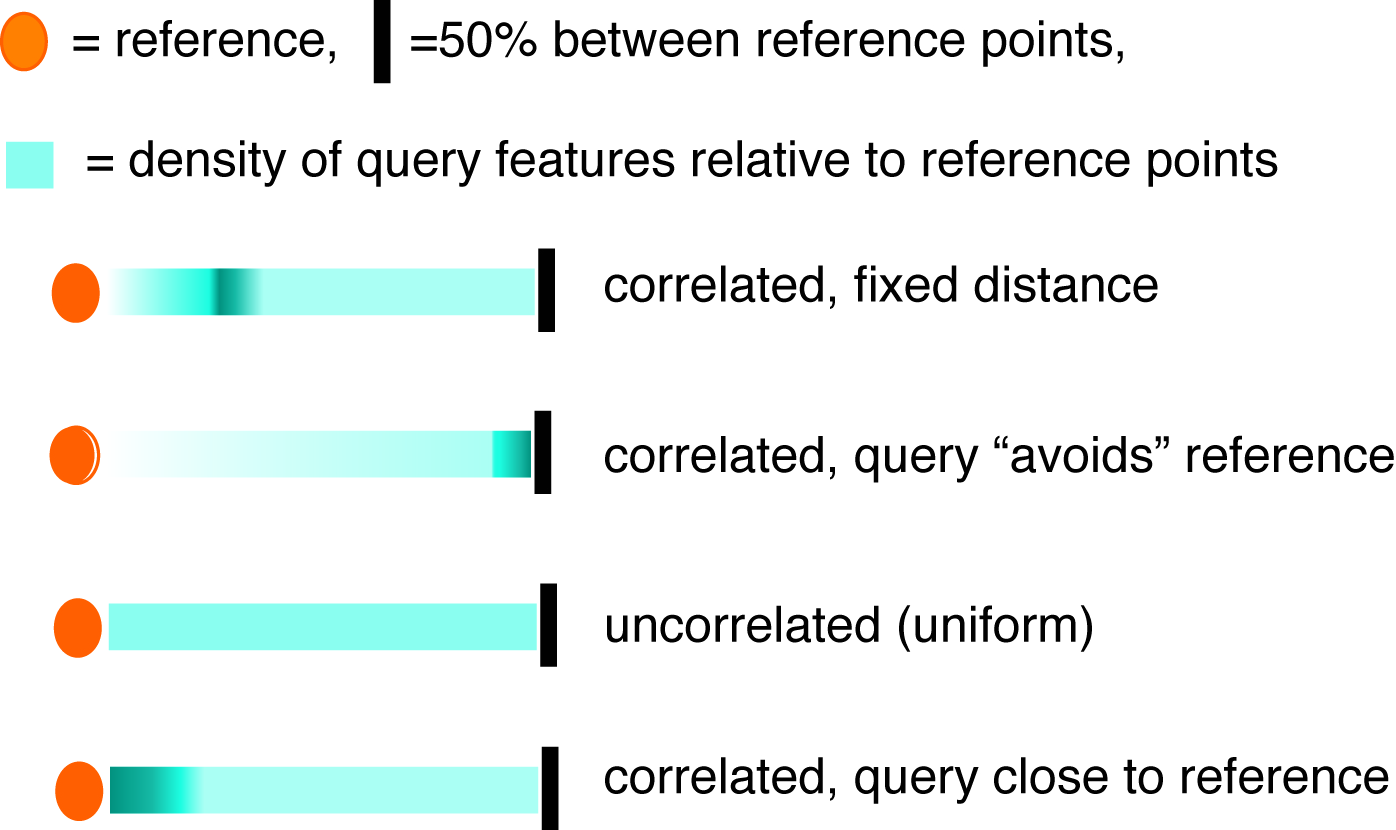
\includegraphics[scale=\picscale]{png/fig3}
	\caption{Our goal is to determine whether the query points are correlated to the reference points. We do this, in essence, by assuming that if they are independent, they will be uniformly distributed with respect to the reference points, and if not, the density of distance between query and reference points will be nonuniform.}
\end{figure*}


Figure 4 illustrates some important complications that we address.


\begin{figure*}[h]
	\centering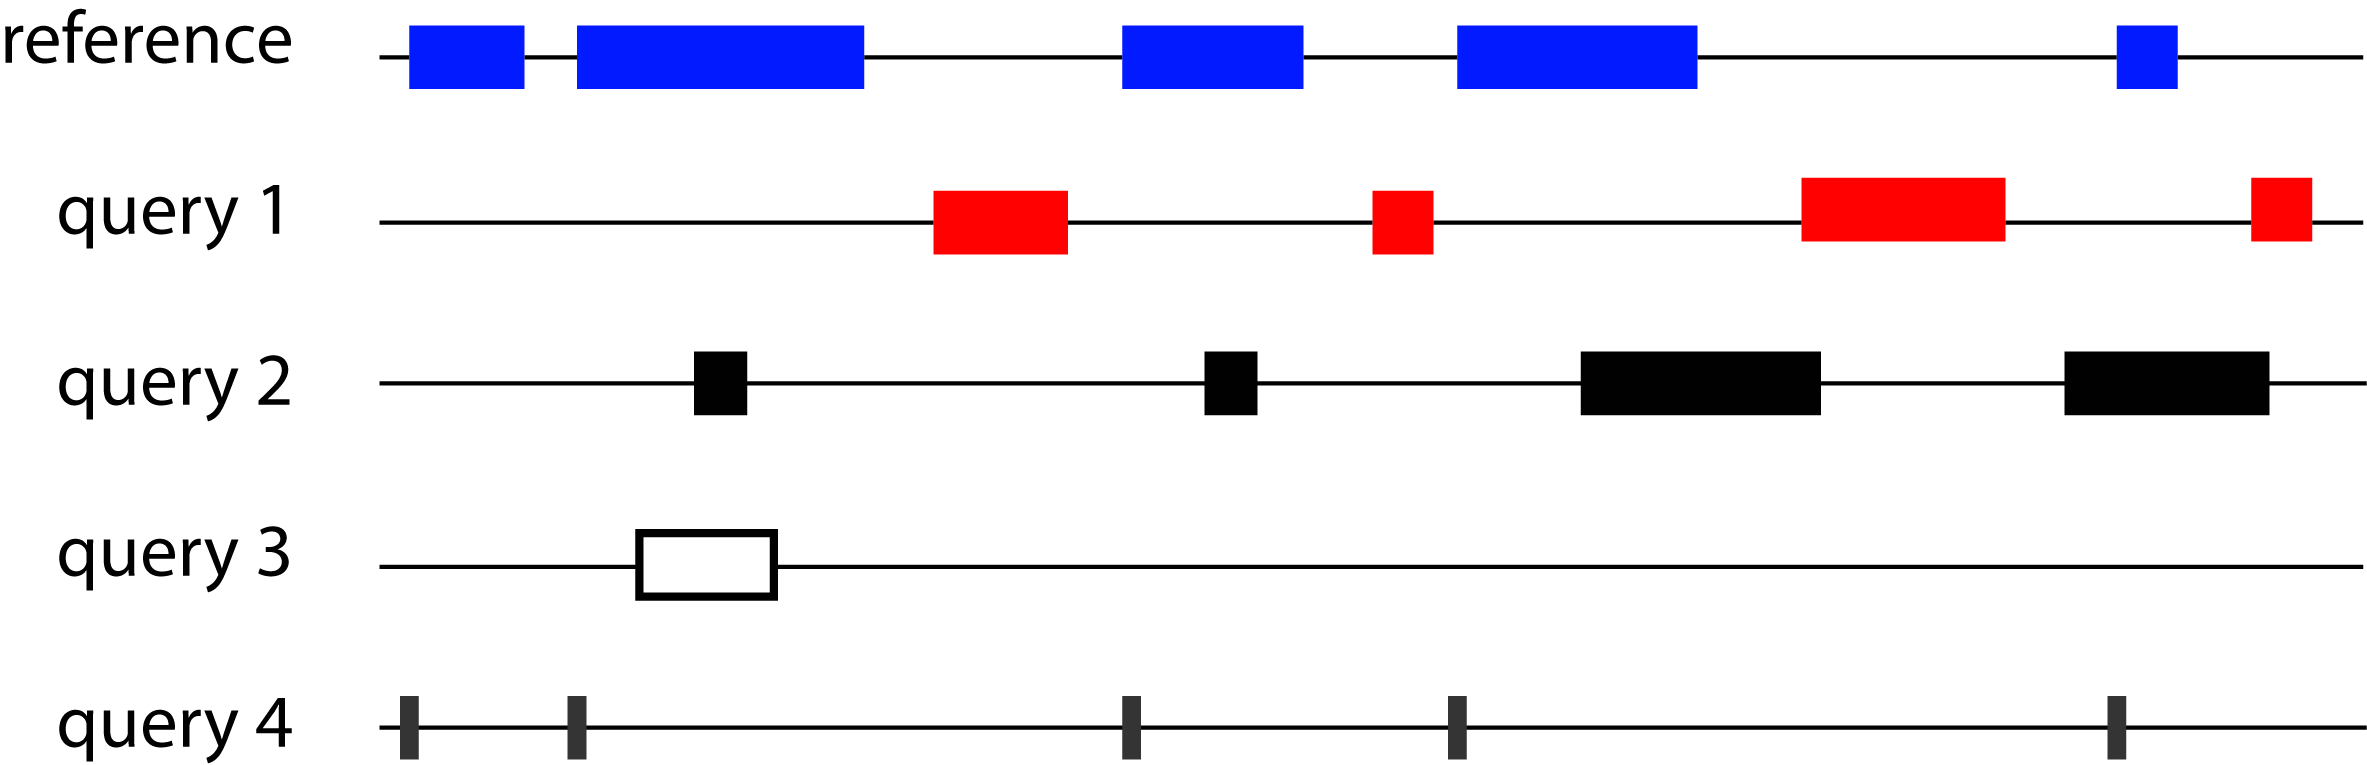
\includegraphics[scale=\picscale]{png/fig4}
	\caption{Four scenarios.}
\end{figure*}
Comparing the intervals in query 1 to the reference intervals, we see that the two sets of intervals consistently do not overlap. They are not independent, and the statistics will show that they are anticorrelated. The query 2 intervals do overlap substantially with the reference intervals and are thus correlated; again the statistics will reflect this and will show a positive association. Query 3 has only one interval. That interval overlaps with a reference interval, so query 3 is correlated with the reference. However, if the query and reference identities are reversed, most of the new query intervals do not overlap with and are not near the single new reference interval, so these two datasets have an asymmetric relationship. Only by testing every query-reference set in both directions can we uncover such an asymmetry. The last set of intervals, query 4, brings up different issues. We can measure the relationship between the query and reference in two ways. First, we can look at the distribution of the midpoints of the query intervals with respect to the distribution of the reference interval midpoints and record the distances as ratios (for example, if the query is 10 units from one reference point and 90 units from the nearest on the other side, its ratio will be 0.1). In a large genome this works well, because average distances are big, so distinguishing a position 10\% into an inverval from a position 30\%
 into an interval is easy. Second, we can look at the raw distance between the midpoints of the query and the midpoints of the reference. This works well for small genomes because here the midpoints of the reference can be close enough that if a query midpoint is, for example, always 100 bp from a reference midpoint, the ratio test will show a much wider distribution, as when the query is between two reference midpoints that are only 300 bp away the ratio test will read 0.33, but when the reference midpoints are 1000 bp away the ratio test will read 0.1, and the query will appear to be uncorrelated. For this reason we find it useful to do both tests, in both directions. These concepts will be elaborated in the next section.

\subsection{Statistical approach}

\subsubsection{Working with intervals}
{\bf Tests on relative distances}

Many of the tests we use work only with pointwise data, not with intervals. Very large intervals may relate to genomic features in different ways, depending on whether we examine their start points, end points, both boundaries, or just a point in the middle. Rather than trying to address this ambiguity or to randomly guess at what the user hopes to do, we expect the user to specify the points when the exact point is important, and we use the midpoint when the user inputs an interval. Also, the user can provide a custom calculation to define the representative point to use for each interval.

Now, we can characterize each query point by its relative distance, as illustrated in figure 5. 

\begin{figure*}[h]
	\centering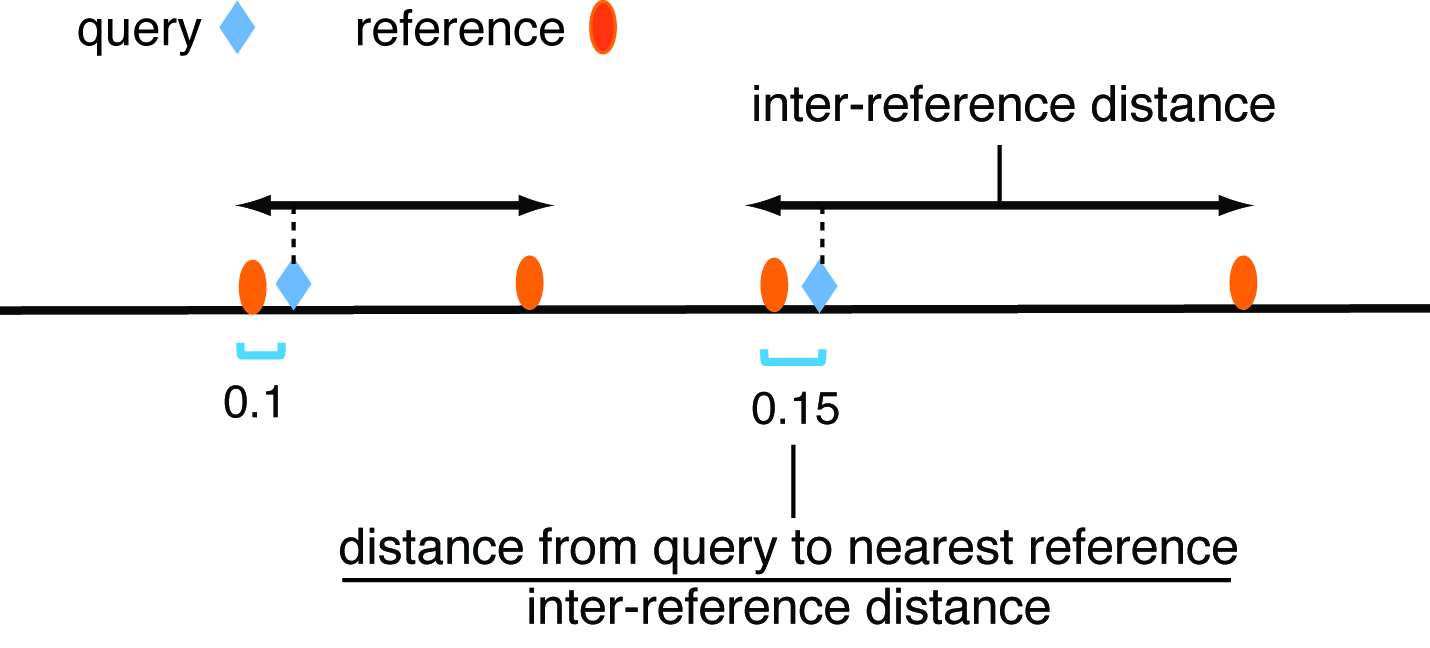
\includegraphics[scale=\picscale]{png/fig5}
	\caption{Relative distance}
\end{figure*}

Formally, the relative distance $d_i$ for a query point $i$ is: 
\[d_i=\displaystyle\frac{\min\left(\left|q_i-r_k\right|,\left|r_{k+1}-q_i\right|\right)}{\left|r_{k+1}-r_k\right|}, k=\arg\min_{q_i \geq r_k}(q_i-r_k).\]

If the reference and query intervals are independent, the query points are positioned randomly with respect to the reference, and the $d_i$'s will be distributed uniformly in $\left[0..0.5\right]$. The corresponding $p-value$ is obtained by using the Kolmogorov-Smirnov test.

\begin{figure*}[h!]
	\centering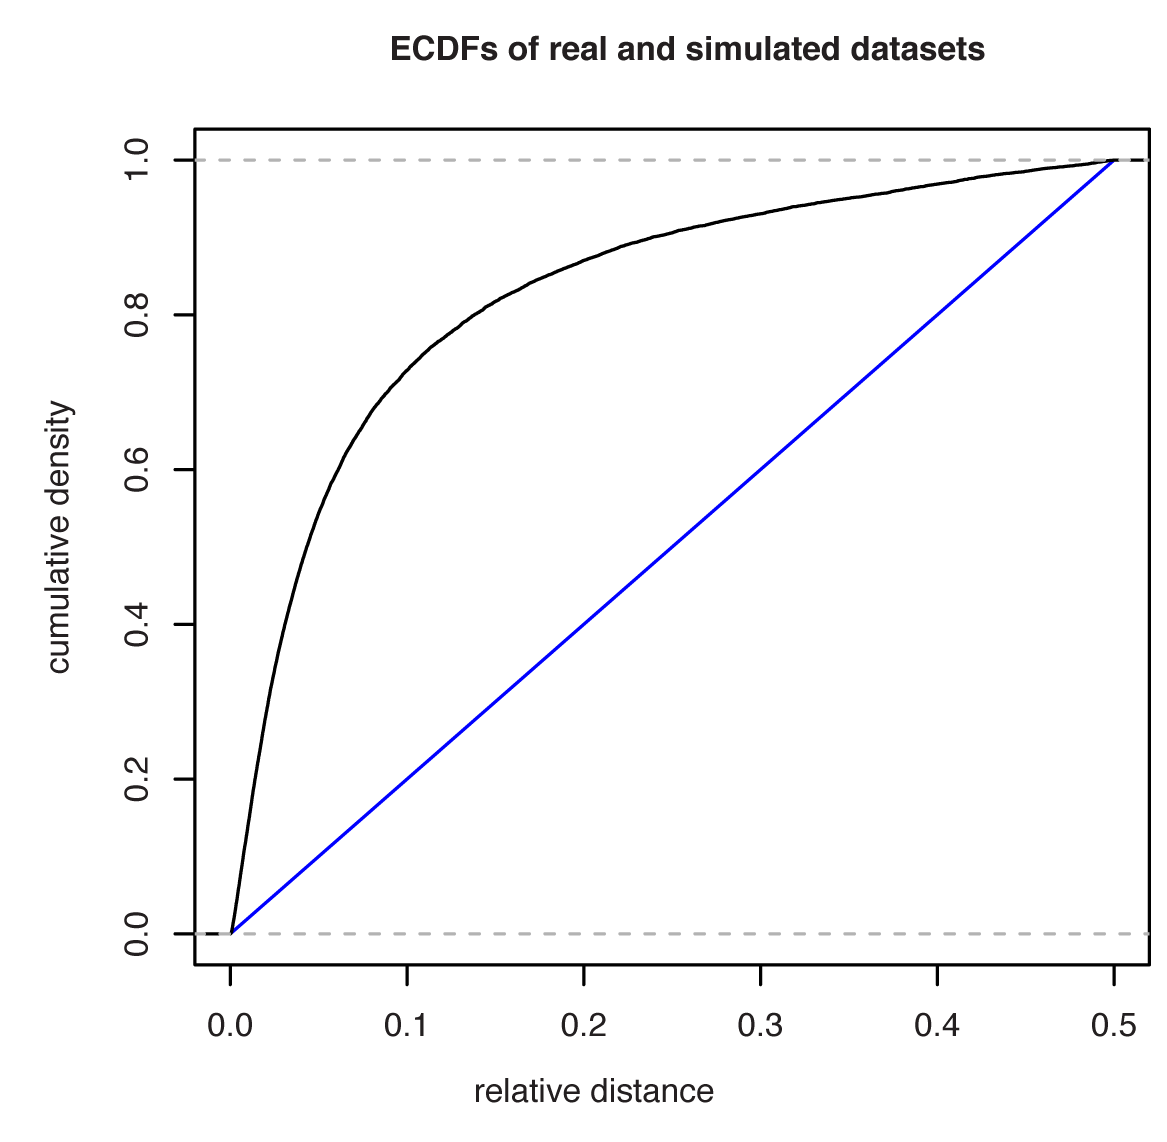
\includegraphics[scale=\picscale]{png/fig6}
	\caption{Area between \textcolor{blue}{uniform ECDF for unrelated feature sets (blue)} and \textcolor{black}{experimental ECDF for related feature sets (black)} is a measure of correlation of the query and reference feature sets.}
\end{figure*}

The Kolmogorov-Smirnov test \(K-S test\) is accompanied by permutation tests to determine the level and direction of deviation from the null expectation. The ECDF (Empirical Distribution Cumulative Function) of the relative distances $d_i$ is a straight line between $(0,0)$ and $(0.5,1)$ if the query and reference points are perfectly independent, so we compare our data to this line.

The area between the ECDF for the reference and query points and the ideal straight line \[S=\displaystyle\int_0^{0.5} \! \left| ECDF(d)-ECDF_{ideal}(d) \right| \, dd \] is a measure of the correlation between the query and reference. So, by drawing $N$ sets of values that model uniform distribution of $d_i$ we get $N$ outcomes of a null distribution for $S$ and thus we can evaluate the $p-value$ for S.   

Both the area permutation test and the Kolmogorov-Smirnov test show only how much the data deviate from independence, not whether they are positively or negatively correlated.

The sign of difference between the areas under the real ECDF curve and the ideal ECDF curve indicates the direction of the correlation. We define a correlation-like measure
\[Corr_{ECDF}=\displaystyle\frac{\displaystyle\int_0^{0.5} \! \left( ECDF(d)-ECDF_{ideal}(d) \right) \, dd}{\displaystyle\int_0^{0.5} \! ECDF_{ideal}(d) \, dd} .\] Positive $Corr_{ECDF}$ indicates positive correlation (query points tend to be close to reference points) and vice versa. 
\definecolor{darkgreen}{RGB}{0,100,0}
\begin{figure*}[h!]
	\centering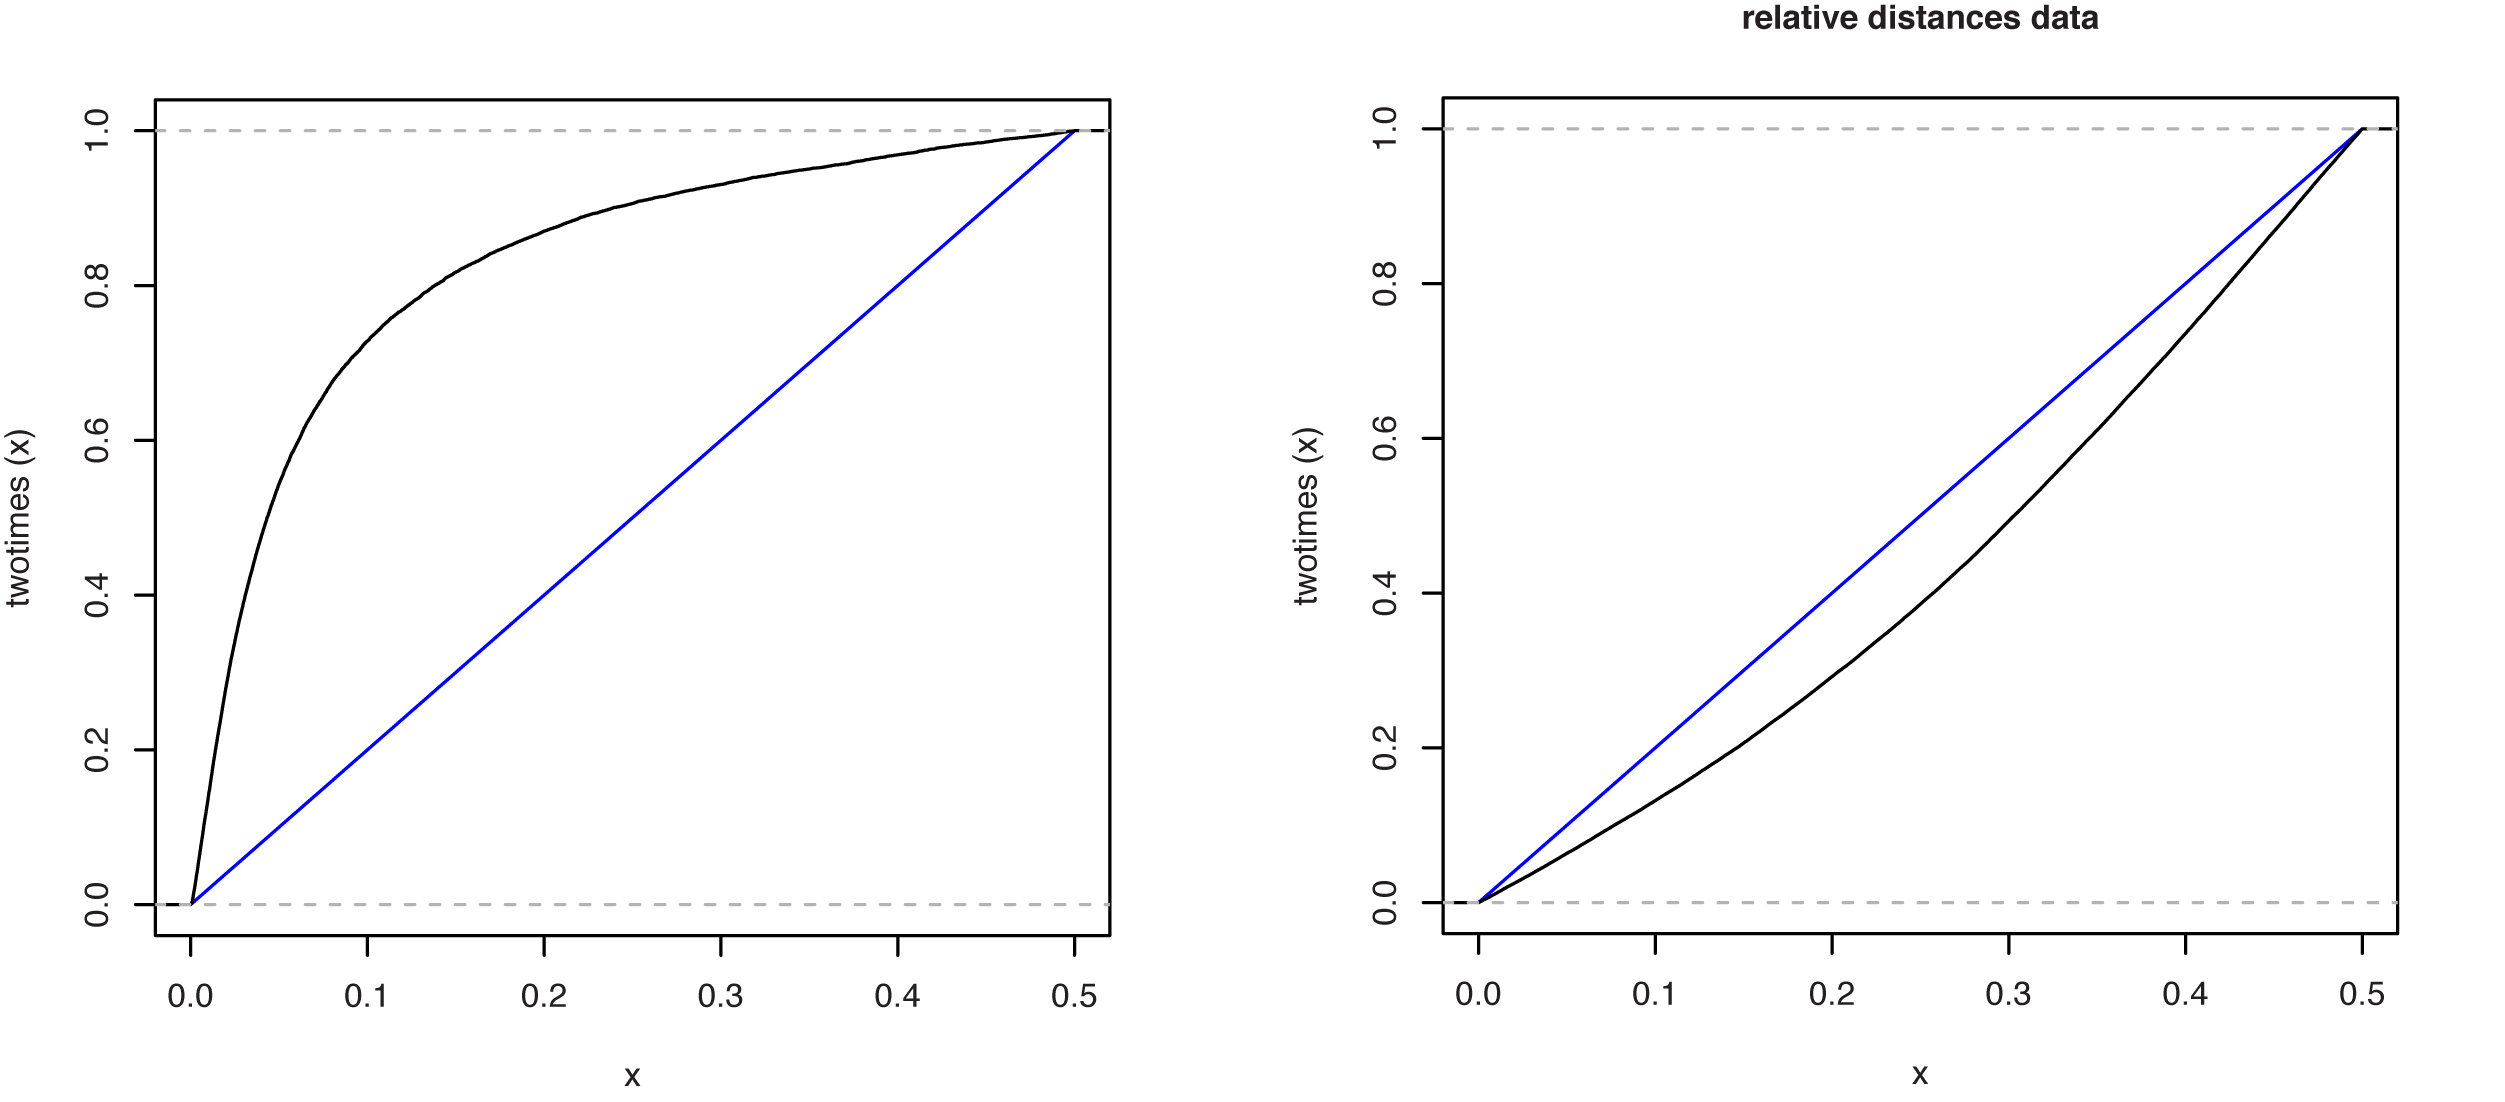
\includegraphics[scale=\picscale]{png/fig7}
	\caption{$Corr_{ECDF}$ is positive for the data represented by the upper black line (left pane); the area under it is more than the area under \textcolor{blue}{the blue line that marks the distribution of independent data}, so the correlation is positive. For the data represented by the lower black line (right pane), the correlation is negative.}
\end{figure*}

\subsubsection{Absolute distance test}
We can also determine whether the query intervals are spaced more often than expected at a specific distance from the reference intervals; for example a polymerase binding site and a transcription factor binding site. Figure 8 illustrates the design.
\begin{figure*}[h!]
        \centering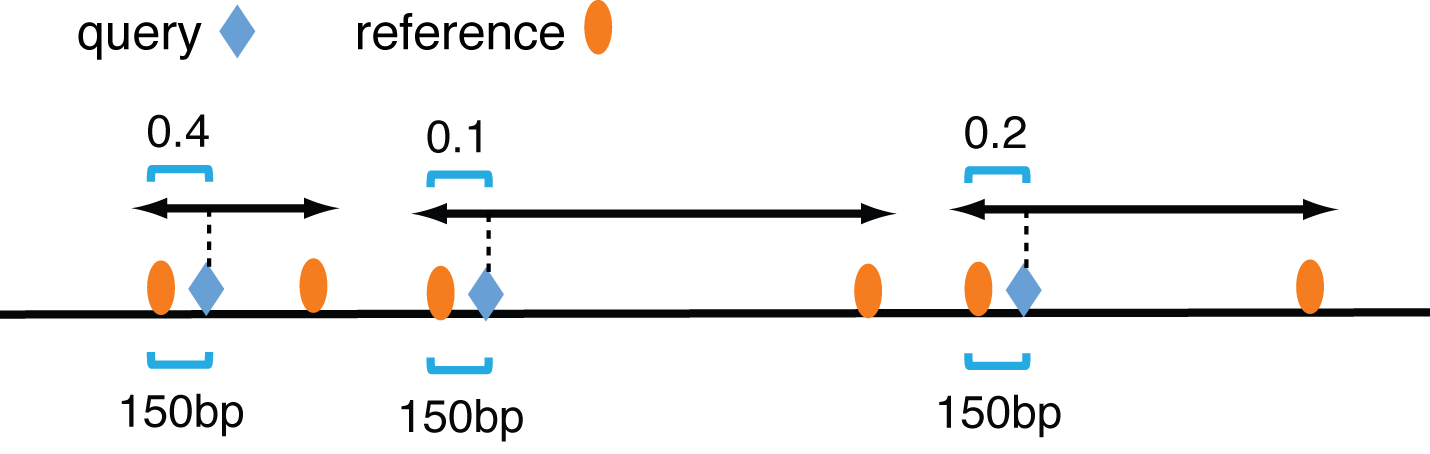
\includegraphics[scale=\picscale]{png/fig8}
        \caption{Query intervals are found at a fixed distance from reference intervals. Relative distances (0.4, 0.1, 0.2) are not consistent.}
\end{figure*}

For each query point (contracted interval) we define the minimal distance to a reference point, $l_i=\min_k(q_i-r_k)$. Its mean value,
\[L=\displaystyle\frac{\displaystyle\sum_i\,l_i}{\#q}\] characterizes the correlation between query and reference points. We perform a permutation test for significance: keeping the reference points fixed, we draw $N$ simulated query positions that are uniformly distributed along the chromosome and calculate $L$ for each, to obtain the null distribution of $L$. The test is two-sided and gives both the $p-value$ for the real $L$, and the sign of any correlation.

\subsubsection{Projection test}

Another test we find useful is the projection test, which is robust when the intervals being tested cover a fairly large percentage of the length of the reference sequence. Here, we determine the number of midpoints of query intervals overlapping the reference intervals and test whether it is outside of the null expectation. The probability of a query midpoint falling into a reference interval is: 
\[p=\displaystyle\frac{\mbox{coverage of the reference}}{\mbox{chromosome length}}\] Therefore, the distribution of the number of query points that overlap reference interval can be approximated by the binomial distribution for $\#q$ trial with success probability $p$. The null hypothesis is that query points hit the reference intervals randomly. The test is also two-sided; it provides both p-value and the direction of correlation.    

\begin{figure*}[h!]
	\centering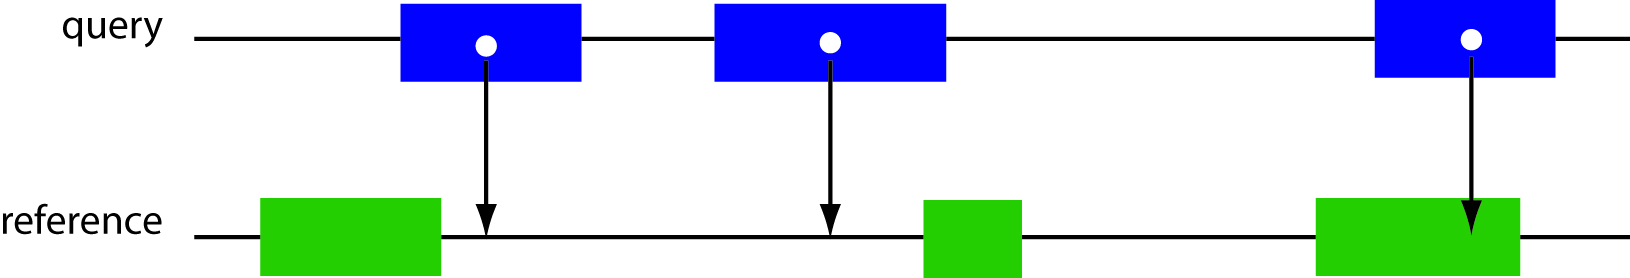
\includegraphics[scale=\picscale]{png/fig9}
	\caption{Projection test.}
\end{figure*}

\subsubsection{Na\"{i}ve Jaccard approach}
\begin{figure*}[h!]
	\centering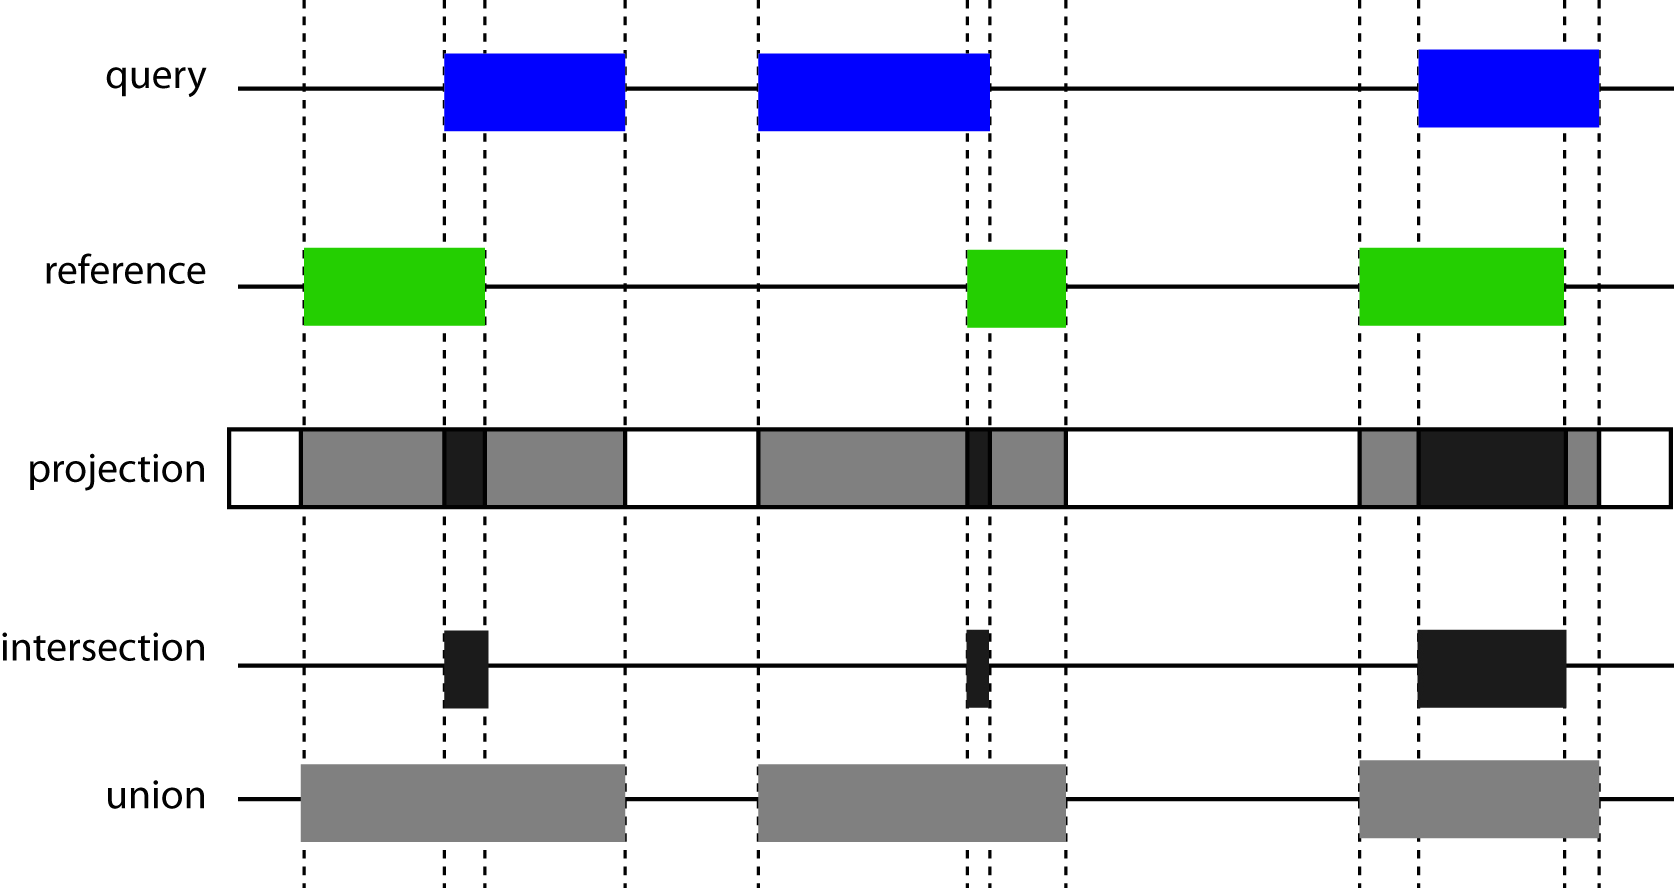
\includegraphics[scale=\picscale]{png/fig10}
	\caption{The Jaccard measure of the correlation of two interval sets is the ratio of the lengths (in bases) of their intersection and their union.}
\end{figure*}
For this we do not test the relationships between points, but between intervals, so this test is quite complementary to the pointwise tests.
\begin{align*}
\mbox{Jaccard measure (index):\ \ } J(A,B)=\displaystyle \frac {A \cap B}{A \cup B}
\end{align*}
To create a null distribution for comparison, we permute the order of the query intervals across the genome, not retaining the lengths of the gaps between the query intervals.


\subsection{Tests of correlation over an entire genome}

All the tests described above are applicable to a single chromosomes or a set of chromosomes (for example, a whole genome). The data for each test are simply summarized over all chromosomes before checking for significance. Another option that is available is restricting the analysis to a set of genomic intervals; for example, asking questions about whether features are correlated when the features always lie within genes is impossible when using the entire genome as the potential space for feature positions, as the features will always look tightly correlated since they co-occur within genes. Using the mapping functions provided, each sub-interval (here, a gene) can be considered as a separate "chromosome," to enable detection of correlations within smaller intervals.


\subsection{GenometriCorr (Genometric Correlation) package}
The package {\tt GenometriCorr} provides functions to load interval data from a plain text file (any accepted format), as well as the main procedure that tests whether the interval sets are spatially independent, and plotting functions to generate graphical representations of the relationships between the features.

\section{Utilities}

\subsection{R objects used by {\tt GenometriCorr}}

The interval sets are represented by the {\tt IRanges} or {\tt RangedData} or {\tt GRanges} objects, which are interval data representation classes defined by {\tt IRanges } package.  {\tt IRanges} is a set of intervals in one space (chromosome). {\tt RangedData} is a set of intervals defined over different spaces (here, chromosomes), so it is suitable for encoding a full-genome annotation.  {\tt GRanges} is very simlar to {\tt RangedData} but it contains the chromosome length information and ensures that operations do not return intervals beyond the length of the chromosomes.

\subsection{Code loading}
Load the package:


\begin{Schunk}
\begin{Sinput}
> library("GenometriCorr")